% flashcards-title: Three equal-length strips cut into halves, fourths, and sixths
% flashcards-desc: Three stacked horizontal strips of identical length, labeled halves, fourths, and sixths on the left. The top strip is cut into two equal parts and its left part is shaded with a pale tint and diagonal hatching; the middle strip is cut into four equal parts; the bottom strip is cut into six equal parts. A dashed vertical guide drops from the right edge of the shaded half through all three strips.
\documentclass[tikz]{standalone}
\usetikzlibrary{arrows.meta,patterns}

\definecolor{qraNavy}{HTML}{17324D}
\definecolor{qraBlue}{HTML}{2B6CB0}
\definecolor{qraGold}{HTML}{B7791F}
\definecolor{qraPale}{HTML}{EAF2F8}
\definecolor{qraGray}{HTML}{5C6773}

\tikzset{
  qra axis/.style={draw=qraNavy, line width=1.2pt},
  qra tick/.style={draw=qraNavy, line width=1pt},
  qra guide/.style={draw=qraGray, densely dashed, line width=0.8pt},
  qra counter/.style={circle, draw=qraNavy, fill=qraPale, line width=0.9pt, minimum size=7mm, inner sep=0pt},
  qra label/.style={font=\sffamily\bfseries, text=qraNavy},
  qra small label/.style={font=\sffamily, text=qraNavy},
}

\begin{document}
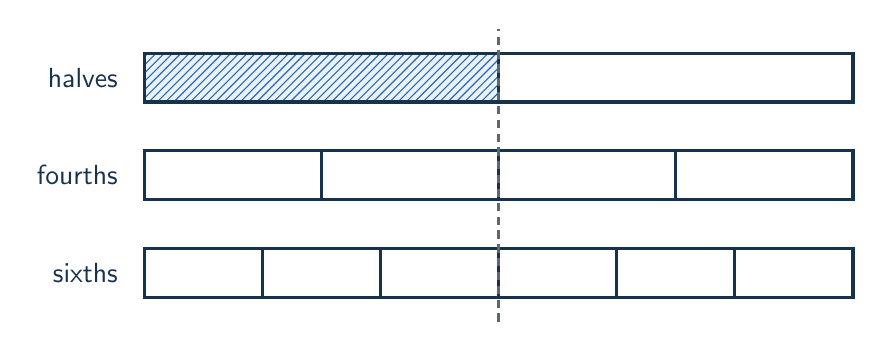
\begin{tikzpicture}[x=1.5cm, y=0.62cm]
  % Top strip: halves, left half shaded
  \fill[qraPale] (0,4) rectangle (3,5);
  \path[pattern=north east lines, pattern color=qraBlue] (0,4) rectangle (3,5);
  \draw[qra tick] (3,4) -- (3,5);
  \draw[qra axis] (0,4) rectangle (6,5);
  \node[qra small label, left=6pt] at (0,4.5) {halves};
  % Middle strip: fourths
  \foreach \i in {1,...,3} \draw[qra tick] ({\i*1.5},2) -- ({\i*1.5},3);
  \draw[qra axis] (0,2) rectangle (6,3);
  \node[qra small label, left=6pt] at (0,2.5) {fourths};
  % Bottom strip: sixths
  \foreach \i in {1,...,5} \draw[qra tick] (\i,0) -- (\i,1);
  \draw[qra axis] (0,0) rectangle (6,1);
  \node[qra small label, left=6pt] at (0,0.5) {sixths};
  % Dashed guide from the shaded boundary through all strips
  \draw[qra guide] (3,-0.5) -- (3,5.5);
\end{tikzpicture}
\end{document}
